\subsection{Структура проекта}

Исходный код приложения представляет из себя Pyhton—проект, разделённый на
логические модули. Такая организация проекта позволяет держать исходный код
в одном репозитории и упростить сборку Python приложения.

Исходный код и используемые в проекте файлы содержатся в корневой папке
\textit{smartcamera}:

\begin{figure}[h!]
  \centering
  \setlength{\fboxsep}{5pt}
  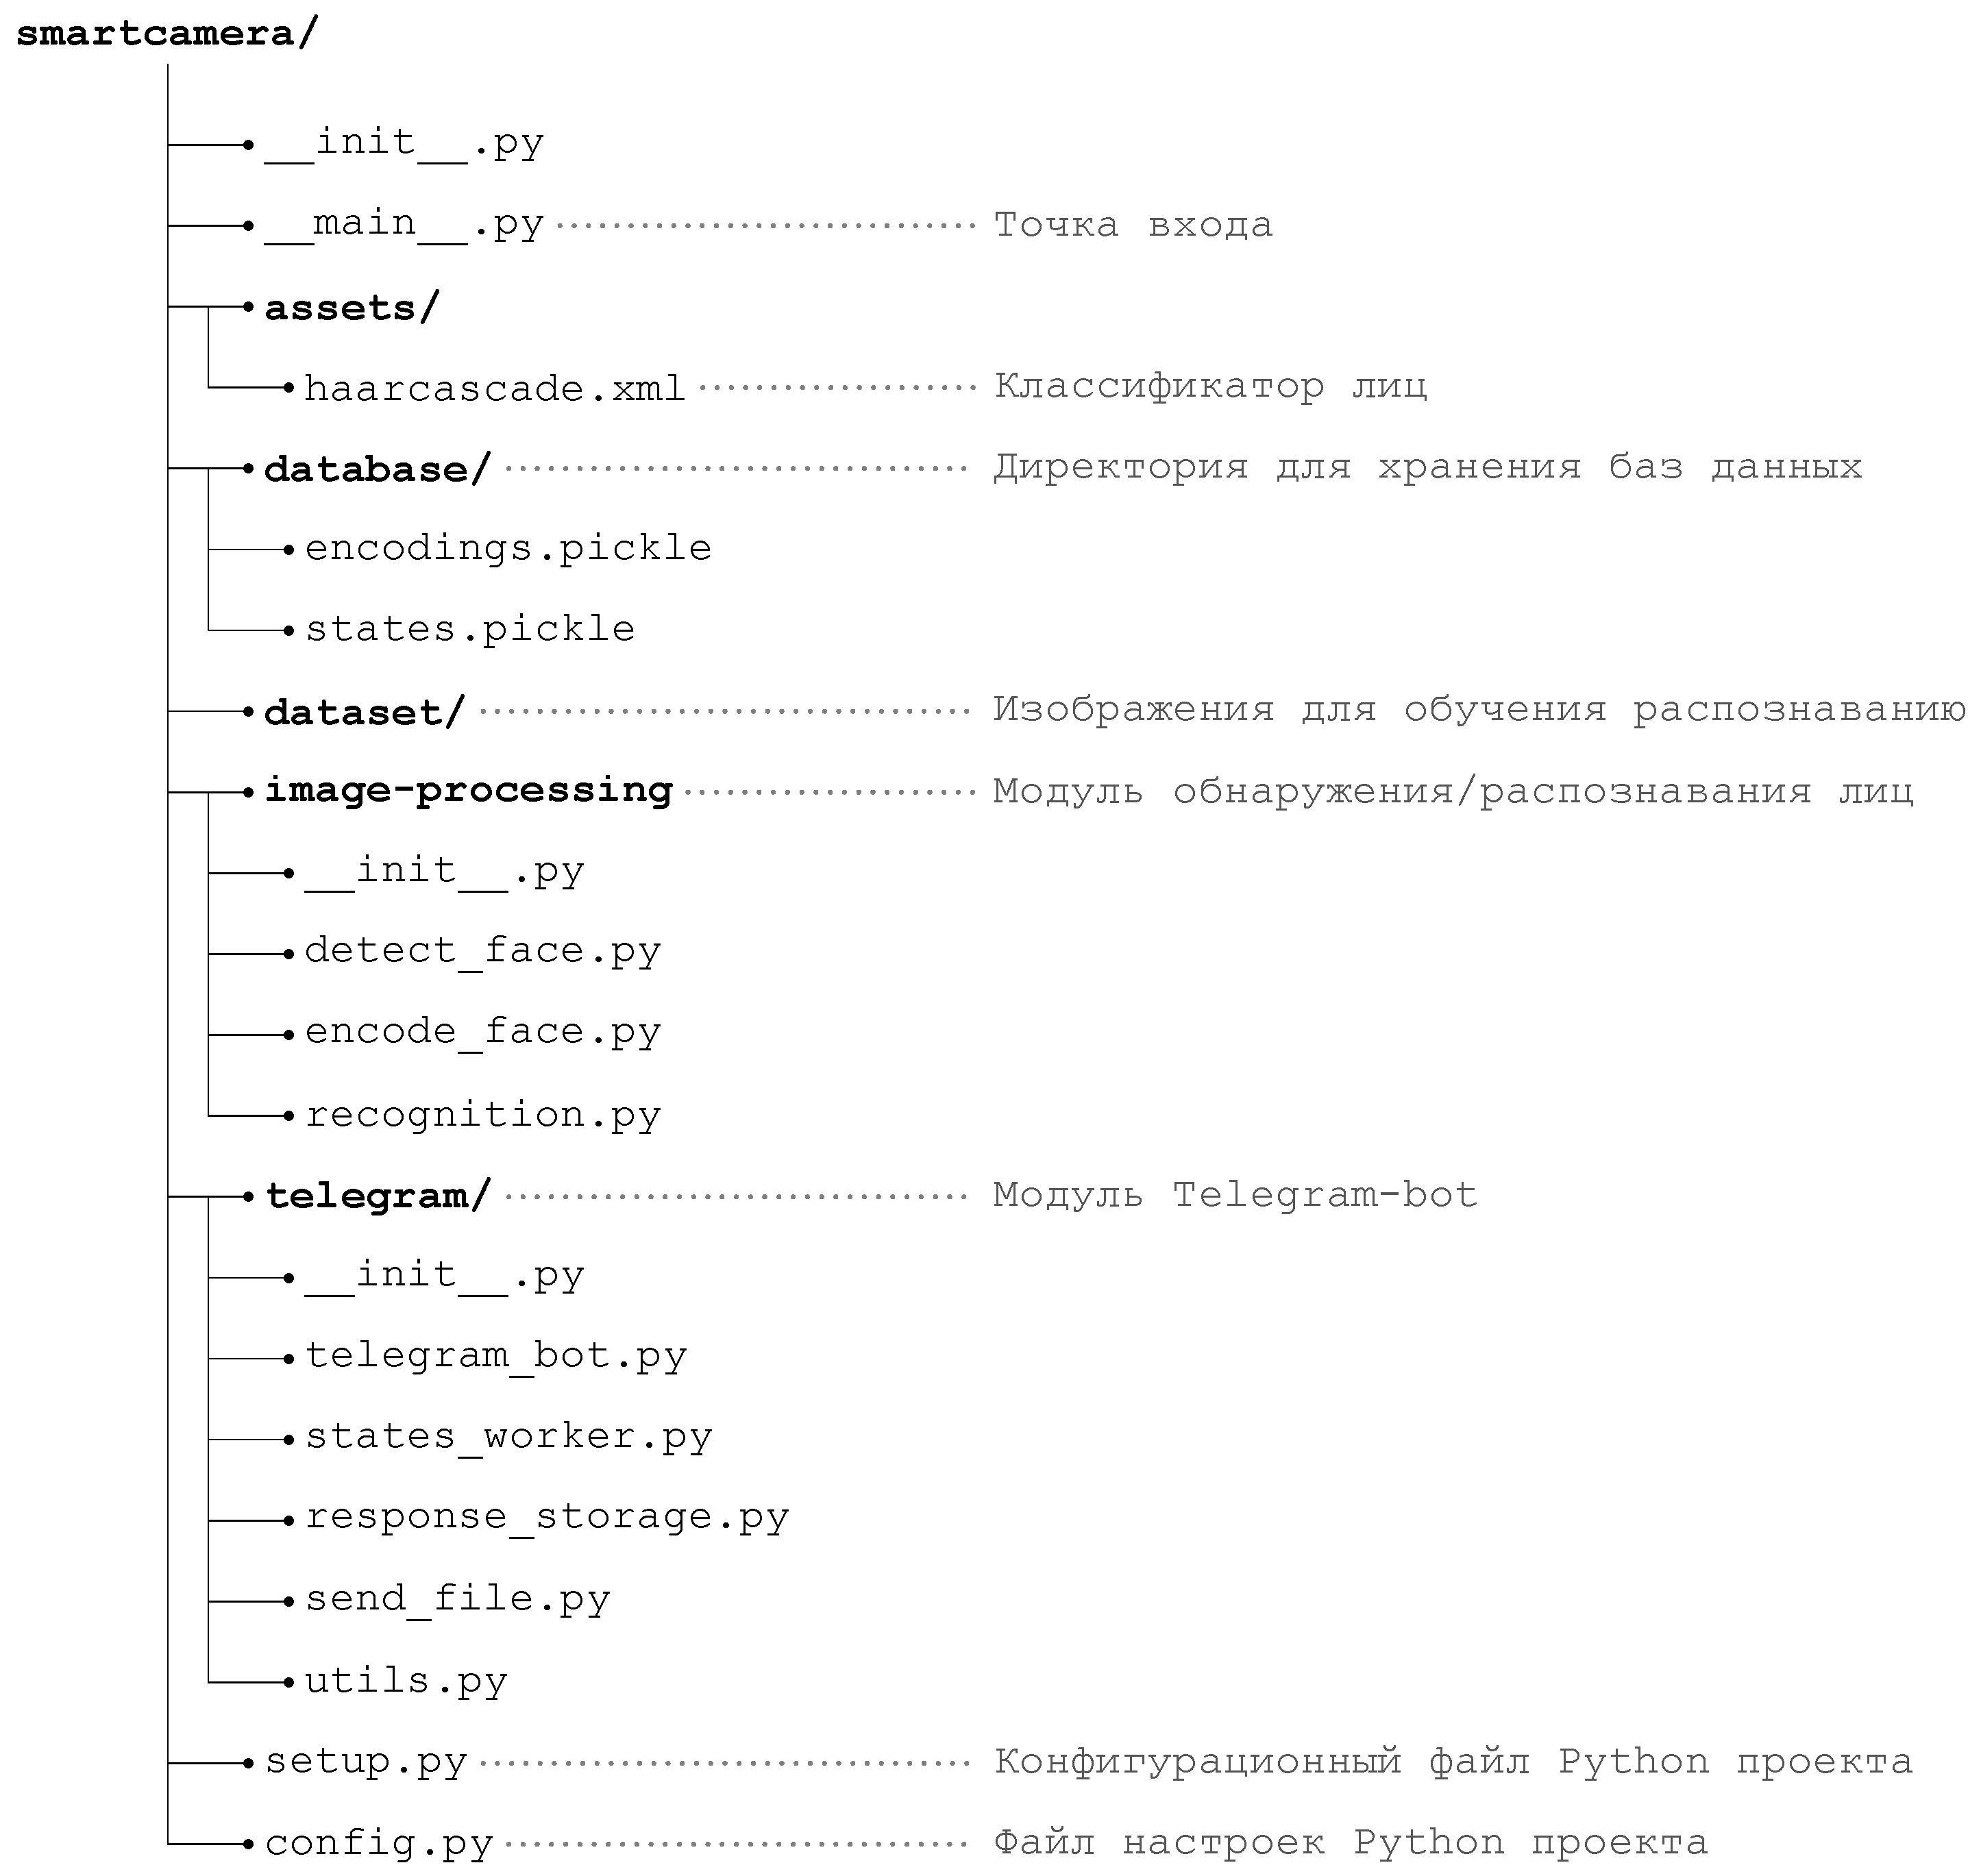
\includegraphics[width=1\textwidth]{data-visualisation/project-tree}
  \vspace*{6pt}
  \caption{Структура проекта}\label{fig:project-tree}
\end{figure}
